\documentclass[1p]{elsarticle_modified}
%\bibliographystyle{elsarticle-num}

%\usepackage[colorlinks]{hyperref}
%\usepackage{abbrmath_seonhwa} %\Abb, \Ascr, \Acal ,\Abf, \Afrak
\usepackage{amsfonts}
\usepackage{amssymb}
\usepackage{amsmath}
\usepackage{amsthm}
\usepackage{scalefnt}
\usepackage{amsbsy}
\usepackage{kotex}
\usepackage{caption}
\usepackage{subfig}
\usepackage{color}
\usepackage{graphicx}
\usepackage{xcolor} %% white, black, red, green, blue, cyan, magenta, yellow
\usepackage{float}
\usepackage{setspace}
\usepackage{hyperref}

\usepackage{tikz}
\usetikzlibrary{arrows}

\usepackage{multirow}
\usepackage{array} % fixed length table
\usepackage{hhline}

%%%%%%%%%%%%%%%%%%%%%
\makeatletter
\renewcommand*\env@matrix[1][\arraystretch]{%
	\edef\arraystretch{#1}%
	\hskip -\arraycolsep
	\let\@ifnextchar\new@ifnextchar
	\array{*\c@MaxMatrixCols c}}
\makeatother %https://tex.stackexchange.com/questions/14071/how-can-i-increase-the-line-spacing-in-a-matrix
%%%%%%%%%%%%%%%

\usepackage[normalem]{ulem}

\newcommand{\msout}[1]{\ifmmode\text{\sout{\ensuremath{#1}}}\else\sout{#1}\fi}
%SOURCE: \msout is \stkout macro in https://tex.stackexchange.com/questions/20609/strikeout-in-math-mode

\newcommand{\cancel}[1]{
	\ifmmode
	{\color{red}\msout{#1}}
	\else
	{\color{red}\sout{#1}}
	\fi
}

\newcommand{\add}[1]{
	{\color{blue}\uwave{#1}}
}

\newcommand{\replace}[2]{
	\ifmmode
	{\color{red}\msout{#1}}{\color{blue}\uwave{#2}}
	\else
	{\color{red}\sout{#1}}{\color{blue}\uwave{#2}}
	\fi
}

\newcommand{\Sol}{\mathcal{S}} %segment
\newcommand{\D}{D} %diagram
\newcommand{\A}{\mathcal{A}} %arc


%%%%%%%%%%%%%%%%%%%%%%%%%%%%%5 test

\def\sl{\operatorname{\textup{SL}}(2,\Cbb)}
\def\psl{\operatorname{\textup{PSL}}(2,\Cbb)}
\def\quan{\mkern 1mu \triangleright \mkern 1mu}

\theoremstyle{definition}
\newtheorem{thm}{Theorem}[section]
\newtheorem{prop}[thm]{Proposition}
\newtheorem{lem}[thm]{Lemma}
\newtheorem{ques}[thm]{Question}
\newtheorem{cor}[thm]{Corollary}
\newtheorem{defn}[thm]{Definition}
\newtheorem{exam}[thm]{Example}
\newtheorem{rmk}[thm]{Remark}
\newtheorem{alg}[thm]{Algorithm}

\newcommand{\I}{\sqrt{-1}}
\begin{document}

%\begin{frontmatter}
%
%\title{Boundary parabolic representations of knots up to 8 crossings}
%
%%% Group authors per affiliation:
%\author{Yunhi Cho} 
%\address{Department of Mathematics, University of Seoul, Seoul, Korea}
%\ead{yhcho@uos.ac.kr}
%
%
%\author{Seonhwa Kim} %\fnref{s_kim}}
%\address{Center for Geometry and Physics, Institute for Basic Science, Pohang, 37673, Korea}
%\ead{ryeona17@ibs.re.kr}
%
%\author{Hyuk Kim}
%\address{Department of Mathematical Sciences, Seoul National University, Seoul 08826, Korea}
%\ead{hyukkim@snu.ac.kr}
%
%\author{Seokbeom Yoon}
%\address{Department of Mathematical Sciences, Seoul National University, Seoul, 08826,  Korea}
%\ead{sbyoon15@snu.ac.kr}
%
%\begin{abstract}
%We find all boundary parabolic representation of knots up to 8 crossings.
%
%\end{abstract}
%\begin{keyword}
%    \MSC[2010] 57M25 
%\end{keyword}
%
%\end{frontmatter}

%\linenumbers
%\tableofcontents
%
\newcommand\colored[1]{\textcolor{white}{\rule[-0.35ex]{0.8em}{1.4ex}}\kern-0.8em\color{red} #1}%
%\newcommand\colored[1]{\textcolor{white}{ #1}\kern-2.17ex	\textcolor{white}{ #1}\kern-1.81ex	\textcolor{white}{ #1}\kern-2.15ex\color{red}#1	}

{\Large $\underline{12a_{0944}~(K12a_{0944})}$}

\setlength{\tabcolsep}{10pt}
\renewcommand{\arraystretch}{1.6}
\vspace{1cm}\begin{tabular}{m{100pt}>{\centering\arraybackslash}m{274pt}}
\multirow{5}{120pt}{
	\centering
	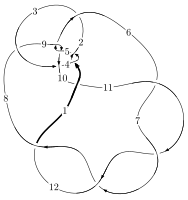
\includegraphics[width=112pt]{../../../GIT/diagram.site/Diagrams/png/1745_12a_0944.png}\\
\ \ \ A knot diagram\footnotemark}&
\allowdisplaybreaks
\textbf{Linearized knot diagam} \\
\cline{2-2}
 &
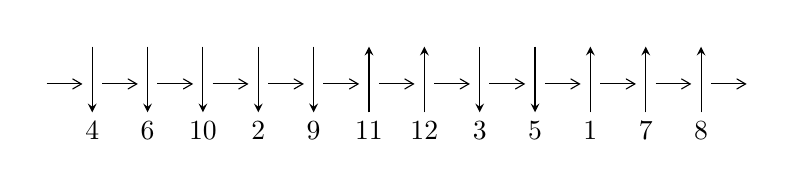
\begin{tikzpicture}[x=20pt, y=17pt]
	% nodes
	\node (C0) at (0, 0) {};
	\node (C1) at (1, 0) {};
	\node (C1U) at (1, +1) {};
	\node (C1D) at (1, -1) {4};

	\node (C2) at (2, 0) {};
	\node (C2U) at (2, +1) {};
	\node (C2D) at (2, -1) {6};

	\node (C3) at (3, 0) {};
	\node (C3U) at (3, +1) {};
	\node (C3D) at (3, -1) {10};

	\node (C4) at (4, 0) {};
	\node (C4U) at (4, +1) {};
	\node (C4D) at (4, -1) {2};

	\node (C5) at (5, 0) {};
	\node (C5U) at (5, +1) {};
	\node (C5D) at (5, -1) {9};

	\node (C6) at (6, 0) {};
	\node (C6U) at (6, +1) {};
	\node (C6D) at (6, -1) {11};

	\node (C7) at (7, 0) {};
	\node (C7U) at (7, +1) {};
	\node (C7D) at (7, -1) {12};

	\node (C8) at (8, 0) {};
	\node (C8U) at (8, +1) {};
	\node (C8D) at (8, -1) {3};

	\node (C9) at (9, 0) {};
	\node (C9U) at (9, +1) {};
	\node (C9D) at (9, -1) {5};

	\node (C10) at (10, 0) {};
	\node (C10U) at (10, +1) {};
	\node (C10D) at (10, -1) {1};

	\node (C11) at (11, 0) {};
	\node (C11U) at (11, +1) {};
	\node (C11D) at (11, -1) {7};

	\node (C12) at (12, 0) {};
	\node (C12U) at (12, +1) {};
	\node (C12D) at (12, -1) {8};
	\node (C13) at (13, 0) {};

	% arrows
	\draw[->,>={angle 60}]
	(C0) edge (C1) (C1) edge (C2) (C2) edge (C3) (C3) edge (C4) (C4) edge (C5) (C5) edge (C6) (C6) edge (C7) (C7) edge (C8) (C8) edge (C9) (C9) edge (C10) (C10) edge (C11) (C11) edge (C12) (C12) edge (C13) ;	\draw[->,>=stealth]
	(C1U) edge (C1D) (C2U) edge (C2D) (C3U) edge (C3D) (C4U) edge (C4D) (C5U) edge (C5D) (C6D) edge (C6U) (C7D) edge (C7U) (C8U) edge (C8D) (C9U) edge (C9D) (C10D) edge (C10U) (C11D) edge (C11U) (C12D) edge (C12U) ;
	\end{tikzpicture} \\
\hhline{~~} \\& 
\textbf{Solving Sequence} \\ \cline{2-2} 
 &
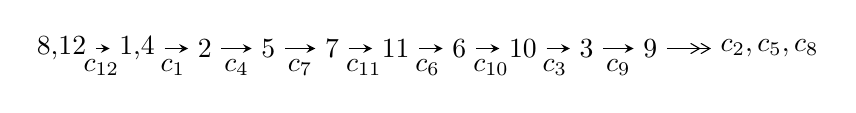
\begin{tikzpicture}[x=23pt, y=7pt]
	% node
	\node (A0) at (-1/8, 0) {8,12};
	\node (A1) at (17/16, 0) {1,4};
	\node (A2) at (17/8, 0) {2};
	\node (A3) at (25/8, 0) {5};
	\node (A4) at (33/8, 0) {7};
	\node (A5) at (41/8, 0) {11};
	\node (A6) at (49/8, 0) {6};
	\node (A7) at (57/8, 0) {10};
	\node (A8) at (65/8, 0) {3};
	\node (A9) at (73/8, 0) {9};
	\node (C1) at (1/2, -1) {$c_{12}$};
	\node (C2) at (13/8, -1) {$c_{1}$};
	\node (C3) at (21/8, -1) {$c_{4}$};
	\node (C4) at (29/8, -1) {$c_{7}$};
	\node (C5) at (37/8, -1) {$c_{11}$};
	\node (C6) at (45/8, -1) {$c_{6}$};
	\node (C7) at (53/8, -1) {$c_{10}$};
	\node (C8) at (61/8, -1) {$c_{3}$};
	\node (C9) at (69/8, -1) {$c_{9}$};
	\node (A10) at (11, 0) {$c_{2},c_{5},c_{8}$};

	% edge
	\draw[->,>=stealth]	
	(A0) edge (A1) (A1) edge (A2) (A2) edge (A3) (A3) edge (A4) (A4) edge (A5) (A5) edge (A6) (A6) edge (A7) (A7) edge (A8) (A8) edge (A9) ;
	\draw[->>,>={angle 60}]	
	(A9) edge (A10);
\end{tikzpicture} \\ 

\end{tabular} \\

\footnotetext{
The image of knot diagram is generated by the software ``\textbf{Draw programme}" developed by Andrew Bartholomew(\url{http://www.layer8.co.uk/maths/draw/index.htm\#Running-draw}), where we modified some parts for our purpose(\url{https://github.com/CATsTAILs/LinksPainter}).
}\phantom \\ \newline 
\centering \textbf{Ideals for irreducible components\footnotemark of $X_{\text{par}}$} 
 
\begin{align*}
I^u_{1}&=\langle 
-5.89366\times10^{43} u^{82}-4.02871\times10^{43} u^{81}+\cdots+5.84962\times10^{43} b-9.28047\times10^{43},\\
\phantom{I^u_{1}}&\phantom{= \langle  }-4.02033\times10^{43} u^{82}-6.96508\times10^{43} u^{81}+\cdots+5.84962\times10^{43} a+9.14712\times10^{42},\;u^{83}+2 u^{82}+\cdots+2 u+1\rangle \\
I^u_{2}&=\langle 
2 b-3,\;2 a+1,\;u-1\rangle \\
\\
\end{align*}
\raggedright * 2 irreducible components of $\dim_{\mathbb{C}}=0$, with total 84 representations.\\
\footnotetext{All coefficients of polynomials are rational numbers. But the coefficients are sometimes approximated in decimal forms when there is not enough margin.}
\newpage
\renewcommand{\arraystretch}{1}
\centering \section*{I. $I^u_{1}= \langle -5.89\times10^{43} u^{82}-4.03\times10^{43} u^{81}+\cdots+5.85\times10^{43} b-9.28\times10^{43},\;-4.02\times10^{43} u^{82}-6.97\times10^{43} u^{81}+\cdots+5.85\times10^{43} a+9.15\times10^{42},\;u^{83}+2 u^{82}+\cdots+2 u+1 \rangle$}
\flushleft \textbf{(i) Arc colorings}\\
\begin{tabular}{m{7pt} m{180pt} m{7pt} m{180pt} }
\flushright $a_{8}=$&$\begin{pmatrix}0\\u\end{pmatrix}$ \\
\flushright $a_{12}=$&$\begin{pmatrix}1\\0\end{pmatrix}$ \\
\flushright $a_{1}=$&$\begin{pmatrix}1\\- u^2\end{pmatrix}$ \\
\flushright $a_{4}=$&$\begin{pmatrix}0.687280 u^{82}+1.19069 u^{81}+\cdots-4.55423 u-0.156371\\1.00753 u^{82}+0.688714 u^{81}+\cdots+2.17242 u+1.58651\end{pmatrix}$ \\
\flushright $a_{2}=$&$\begin{pmatrix}0.595958 u^{82}+0.451262 u^{81}+\cdots-3.44105 u+1.45422\\0.130801 u^{82}+0.302832 u^{81}+\cdots+0.730664 u+0.811722\end{pmatrix}$ \\
\flushright $a_{5}=$&$\begin{pmatrix}0.485737 u^{82}+1.80641 u^{81}+\cdots-1.46200 u-1.94018\\1.01774 u^{82}+0.0762026 u^{81}+\cdots+2.45408 u+1.22439\end{pmatrix}$ \\
\flushright $a_{7}=$&$\begin{pmatrix}- u\\u\end{pmatrix}$ \\
\flushright $a_{11}=$&$\begin{pmatrix}- u^2+1\\u^2\end{pmatrix}$ \\
\flushright $a_{6}=$&$\begin{pmatrix}u^3-2 u\\- u^3+u\end{pmatrix}$ \\
\flushright $a_{10}=$&$\begin{pmatrix}u^4-3 u^2+1\\- u^6+2 u^4+u^2\end{pmatrix}$ \\
\flushright $a_{3}=$&$\begin{pmatrix}-0.0563813 u^{82}-0.557025 u^{81}+\cdots-0.575560 u+2.07556\\1.78385 u^{82}+1.83521 u^{81}+\cdots+0.274886 u+1.23971\end{pmatrix}$ \\
\flushright $a_{9}=$&$\begin{pmatrix}0.389463 u^{82}+0.804666 u^{81}+\cdots-2.31500 u+0.480446\\0.263809 u^{82}-0.0637110 u^{81}+\cdots-2.47071 u-0.459997\end{pmatrix}$\\&\end{tabular}
\flushleft \textbf{(ii) Obstruction class $= -1$}\\~\\
\flushleft \textbf{(iii) Cusp Shapes $= 0.357481 u^{82}-3.48793 u^{81}+\cdots+11.5669 u-5.41910$}\\~\\
\newpage\renewcommand{\arraystretch}{1}
\flushleft \textbf{(iv) u-Polynomials at the component}\newline \\
\begin{tabular}{m{50pt}|m{274pt}}
Crossings & \hspace{64pt}u-Polynomials at each crossing \\
\hline $$\begin{aligned}c_{1},c_{4}\end{aligned}$$&$\begin{aligned}
&u^{83}-2 u^{82}+\cdots-35 u+4
\end{aligned}$\\
\hline $$\begin{aligned}c_{2}\end{aligned}$$&$\begin{aligned}
&2(2 u^{83}-13 u^{82}+\cdots+3 u+1)
\end{aligned}$\\
\hline $$\begin{aligned}c_{3}\end{aligned}$$&$\begin{aligned}
&2(2 u^{83}-11 u^{82}+\cdots+4480 u+352)
\end{aligned}$\\
\hline $$\begin{aligned}c_{5},c_{9}\end{aligned}$$&$\begin{aligned}
&u^{83}+2 u^{82}+\cdots+4 u+1
\end{aligned}$\\
\hline $$\begin{aligned}c_{6},c_{7},c_{11}\\c_{12}\end{aligned}$$&$\begin{aligned}
&u^{83}+2 u^{82}+\cdots+2 u+1
\end{aligned}$\\
\hline $$\begin{aligned}c_{8}\end{aligned}$$&$\begin{aligned}
&u^{83}+u^{82}+\cdots-2 u+8
\end{aligned}$\\
\hline $$\begin{aligned}c_{10}\end{aligned}$$&$\begin{aligned}
&u^{83}+16 u^{82}+\cdots-11522 u-2671
\end{aligned}$\\
\hline
\end{tabular}\\~\\
\newpage\renewcommand{\arraystretch}{1}
\flushleft \textbf{(v) Riley Polynomials at the component}\newline \\
\begin{tabular}{m{50pt}|m{274pt}}
Crossings & \hspace{64pt}Riley Polynomials at each crossing \\
\hline $$\begin{aligned}c_{1},c_{4}\end{aligned}$$&$\begin{aligned}
&y^{83}-52 y^{82}+\cdots-479 y-16
\end{aligned}$\\
\hline $$\begin{aligned}c_{2}\end{aligned}$$&$\begin{aligned}
&4(4 y^{83}+523 y^{82}+\cdots-117 y-1)
\end{aligned}$\\
\hline $$\begin{aligned}c_{3}\end{aligned}$$&$\begin{aligned}
&4(4 y^{83}-517 y^{82}+\cdots+6829568 y-123904)
\end{aligned}$\\
\hline $$\begin{aligned}c_{5},c_{9}\end{aligned}$$&$\begin{aligned}
&y^{83}+48 y^{82}+\cdots+12 y-1
\end{aligned}$\\
\hline $$\begin{aligned}c_{6},c_{7},c_{11}\\c_{12}\end{aligned}$$&$\begin{aligned}
&y^{83}-92 y^{82}+\cdots+12 y-1
\end{aligned}$\\
\hline $$\begin{aligned}c_{8}\end{aligned}$$&$\begin{aligned}
&y^{83}+9 y^{82}+\cdots+2164 y-64
\end{aligned}$\\
\hline $$\begin{aligned}c_{10}\end{aligned}$$&$\begin{aligned}
&y^{83}+28 y^{82}+\cdots+65725068 y-7134241
\end{aligned}$\\
\hline
\end{tabular}\\~\\
\newpage\flushleft \textbf{(vi) Complex Volumes and Cusp Shapes}
$$\begin{array}{c|c|c}  
\text{Solutions to }I^u_{1}& \I (\text{vol} + \sqrt{-1}CS) & \text{Cusp shape}\\
 \hline 
\begin{aligned}
u &= -1.011980 + 0.179958 I \\
a &= \phantom{-}0.609871 - 0.498601 I \\
b &= -1.54206 + 0.26964 I\end{aligned}
 & \phantom{-}3.08858 - 7.00447 I & \phantom{-0.000000 } 0 \\ \hline\begin{aligned}
u &= -1.011980 - 0.179958 I \\
a &= \phantom{-}0.609871 + 0.498601 I \\
b &= -1.54206 - 0.26964 I\end{aligned}
 & \phantom{-}3.08858 + 7.00447 I & \phantom{-0.000000 } 0 \\ \hline\begin{aligned}
u &= \phantom{-}0.808275 + 0.494108 I \\
a &= \phantom{-}0.668900 + 0.762033 I \\
b &= -0.506716 - 0.978105 I\end{aligned}
 & \phantom{-}1.080250 + 0.304022 I & \phantom{-0.000000 } 0 \\ \hline\begin{aligned}
u &= \phantom{-}0.808275 - 0.494108 I \\
a &= \phantom{-}0.668900 - 0.762033 I \\
b &= -0.506716 + 0.978105 I\end{aligned}
 & \phantom{-}1.080250 - 0.304022 I & \phantom{-0.000000 } 0 \\ \hline\begin{aligned}
u &= -0.651779 + 0.604556 I \\
a &= \phantom{-}1.96345 - 1.28262 I \\
b &= -0.373780 + 1.237280 I\end{aligned}
 & -4.75200 - 7.90588 I & \phantom{-0.000000 } 0 \\ \hline\begin{aligned}
u &= -0.651779 - 0.604556 I \\
a &= \phantom{-}1.96345 + 1.28262 I \\
b &= -0.373780 - 1.237280 I\end{aligned}
 & -4.75200 + 7.90588 I & \phantom{-0.000000 } 0 \\ \hline\begin{aligned}
u &= \phantom{-}0.651416 + 0.587957 I \\
a &= \phantom{-}2.25811 + 1.40134 I \\
b &= -0.455813 - 1.238970 I\end{aligned}
 & -1.07019 + 13.90660 I & \phantom{-0.000000 } 0 \\ \hline\begin{aligned}
u &= \phantom{-}0.651416 - 0.587957 I \\
a &= \phantom{-}2.25811 - 1.40134 I \\
b &= -0.455813 + 1.238970 I\end{aligned}
 & -1.07019 - 13.90660 I & \phantom{-0.000000 } 0 \\ \hline\begin{aligned}
u &= \phantom{-}0.549669 + 0.652540 I \\
a &= \phantom{-}1.77757 + 0.60916 I \\
b &= -0.166242 - 1.069510 I\end{aligned}
 & \phantom{-}1.14584 + 2.23192 I & \phantom{-0.000000 } 0 \\ \hline\begin{aligned}
u &= \phantom{-}0.549669 - 0.652540 I \\
a &= \phantom{-}1.77757 - 0.60916 I \\
b &= -0.166242 + 1.069510 I\end{aligned}
 & \phantom{-}1.14584 - 2.23192 I & \phantom{-0.000000 } 0\\
 \hline 
 \end{array}$$\newpage$$\begin{array}{c|c|c}  
\text{Solutions to }I^u_{1}& \I (\text{vol} + \sqrt{-1}CS) & \text{Cusp shape}\\
 \hline 
\begin{aligned}
u &= \phantom{-}0.621208 + 0.516711 I \\
a &= -1.122620 + 0.653975 I \\
b &= \phantom{-}0.442519 - 0.591802 I\end{aligned}
 & \phantom{-}2.87214 + 7.55799 I & \phantom{-0.000000 } 0. - 9.17056 I \\ \hline\begin{aligned}
u &= \phantom{-}0.621208 - 0.516711 I \\
a &= -1.122620 - 0.653975 I \\
b &= \phantom{-}0.442519 + 0.591802 I\end{aligned}
 & \phantom{-}2.87214 - 7.55799 I & \phantom{-0.000000 -}0. + 9.17056 I \\ \hline\begin{aligned}
u &= -0.794140 + 0.067445 I \\
a &= \phantom{-}0.828496 - 0.746859 I \\
b &= -0.754413 - 0.297712 I\end{aligned}
 & \phantom{-}5.68714 + 2.25774 I & \phantom{-}7.48178 - 1.40093 I \\ \hline\begin{aligned}
u &= -0.794140 - 0.067445 I \\
a &= \phantom{-}0.828496 + 0.746859 I \\
b &= -0.754413 + 0.297712 I\end{aligned}
 & \phantom{-}5.68714 - 2.25774 I & \phantom{-}7.48178 + 1.40093 I \\ \hline\begin{aligned}
u &= -0.603519 + 0.480975 I \\
a &= -0.693273 + 0.188096 I \\
b &= \phantom{-}0.158367 + 0.299299 I\end{aligned}
 & -0.49436 - 3.88362 I & -2.00000 + 7.10699 I \\ \hline\begin{aligned}
u &= -0.603519 - 0.480975 I \\
a &= -0.693273 - 0.188096 I \\
b &= \phantom{-}0.158367 - 0.299299 I\end{aligned}
 & -0.49436 + 3.88362 I & -2.00000 - 7.10699 I \\ \hline\begin{aligned}
u &= -0.311368 + 0.686203 I \\
a &= \phantom{-}2.05458 - 0.49843 I \\
b &= -0.259155 + 0.996903 I\end{aligned}
 & -5.76402 + 3.56956 I & -7.33230 - 3.19643 I \\ \hline\begin{aligned}
u &= -0.311368 - 0.686203 I \\
a &= \phantom{-}2.05458 + 0.49843 I \\
b &= -0.259155 - 0.996903 I\end{aligned}
 & -5.76402 - 3.56956 I & -7.33230 + 3.19643 I \\ \hline\begin{aligned}
u &= -0.540900 + 0.513654 I \\
a &= -2.36141 + 1.14016 I \\
b &= \phantom{-}0.686576 - 0.514783 I\end{aligned}
 & -2.34688 - 5.23319 I & -4.54446 + 9.84503 I \\ \hline\begin{aligned}
u &= -0.540900 - 0.513654 I \\
a &= -2.36141 - 1.14016 I \\
b &= \phantom{-}0.686576 + 0.514783 I\end{aligned}
 & -2.34688 + 5.23319 I & -4.54446 - 9.84503 I\\
 \hline 
 \end{array}$$\newpage$$\begin{array}{c|c|c}  
\text{Solutions to }I^u_{1}& \I (\text{vol} + \sqrt{-1}CS) & \text{Cusp shape}\\
 \hline 
\begin{aligned}
u &= \phantom{-}0.302357 + 0.661044 I \\
a &= \phantom{-}2.15568 + 0.69658 I \\
b &= -0.305424 - 1.170910 I\end{aligned}
 & -2.10269 - 9.69142 I & -3.57256 + 4.73391 I \\ \hline\begin{aligned}
u &= \phantom{-}0.302357 - 0.661044 I \\
a &= \phantom{-}2.15568 - 0.69658 I \\
b &= -0.305424 + 1.170910 I\end{aligned}
 & -2.10269 + 9.69142 I & -3.57256 - 4.73391 I \\ \hline\begin{aligned}
u &= \phantom{-}0.176369 + 0.694417 I \\
a &= \phantom{-}1.79640 - 0.14808 I \\
b &= -0.244225 - 0.252132 I\end{aligned}
 & -0.84399 + 3.83418 I & -2.64069 - 10.16954 I \\ \hline\begin{aligned}
u &= \phantom{-}0.176369 - 0.694417 I \\
a &= \phantom{-}1.79640 + 0.14808 I \\
b &= -0.244225 + 0.252132 I\end{aligned}
 & -0.84399 - 3.83418 I & -2.64069 + 10.16954 I \\ \hline\begin{aligned}
u &= \phantom{-}0.659821 + 0.267940 I \\
a &= \phantom{-}0.761044 + 0.351679 I \\
b &= -0.382761 - 0.240353 I\end{aligned}
 & \phantom{-}1.22968 + 0.74629 I & \phantom{-}5.11191 - 1.69537 I \\ \hline\begin{aligned}
u &= \phantom{-}0.659821 - 0.267940 I \\
a &= \phantom{-}0.761044 - 0.351679 I \\
b &= -0.382761 + 0.240353 I\end{aligned}
 & \phantom{-}1.22968 - 0.74629 I & \phantom{-}5.11191 + 1.69537 I \\ \hline\begin{aligned}
u &= \phantom{-}0.501968 + 0.498745 I \\
a &= -2.65030 - 1.61037 I \\
b &= \phantom{-}0.629147 + 1.068660 I\end{aligned}
 & -3.50723 + 1.89136 I & -6.82387 - 2.66530 I \\ \hline\begin{aligned}
u &= \phantom{-}0.501968 - 0.498745 I \\
a &= -2.65030 + 1.61037 I \\
b &= \phantom{-}0.629147 - 1.068660 I\end{aligned}
 & -3.50723 - 1.89136 I & -6.82387 + 2.66530 I \\ \hline\begin{aligned}
u &= \phantom{-}1.289970 + 0.207695 I \\
a &= \phantom{-}0.815121 + 0.281289 I \\
b &= -2.32584 - 1.05852 I\end{aligned}
 & -0.716216 - 0.352949 I & \phantom{-0.000000 } 0 \\ \hline\begin{aligned}
u &= \phantom{-}1.289970 - 0.207695 I \\
a &= \phantom{-}0.815121 - 0.281289 I \\
b &= -2.32584 + 1.05852 I\end{aligned}
 & -0.716216 + 0.352949 I & \phantom{-0.000000 } 0\\
 \hline 
 \end{array}$$\newpage$$\begin{array}{c|c|c}  
\text{Solutions to }I^u_{1}& \I (\text{vol} + \sqrt{-1}CS) & \text{Cusp shape}\\
 \hline 
\begin{aligned}
u &= -1.305710 + 0.116254 I \\
a &= \phantom{-}0.821552 - 0.148933 I \\
b &= -2.60864 + 0.95083 I\end{aligned}
 & \phantom{-}2.88394 + 6.80535 I & \phantom{-0.000000 } 0 \\ \hline\begin{aligned}
u &= -1.305710 - 0.116254 I \\
a &= \phantom{-}0.821552 + 0.148933 I \\
b &= -2.60864 - 0.95083 I\end{aligned}
 & \phantom{-}2.88394 - 6.80535 I & \phantom{-0.000000 } 0 \\ \hline\begin{aligned}
u &= \phantom{-}0.465968 + 0.499477 I \\
a &= -2.48917 - 1.39113 I \\
b &= \phantom{-}0.76305 + 1.24356 I\end{aligned}
 & -3.61323 + 1.60159 I & -7.16367 - 5.67884 I \\ \hline\begin{aligned}
u &= \phantom{-}0.465968 - 0.499477 I \\
a &= -2.48917 + 1.39113 I \\
b &= \phantom{-}0.76305 - 1.24356 I\end{aligned}
 & -3.61323 - 1.60159 I & -7.16367 + 5.67884 I \\ \hline\begin{aligned}
u &= -0.533295 + 0.405202 I \\
a &= \phantom{-}3.22952 + 9.36950 I \\
b &= -3.45923 + 0.25484 I\end{aligned}
 & -0.168100 - 1.376260 I & -60.2145 + 47.3401 I \\ \hline\begin{aligned}
u &= -0.533295 - 0.405202 I \\
a &= \phantom{-}3.22952 - 9.36950 I \\
b &= -3.45923 - 0.25484 I\end{aligned}
 & -0.168100 + 1.376260 I & -60.2145 - 47.3401 I \\ \hline\begin{aligned}
u &= -0.413981 + 0.510073 I \\
a &= -1.43503 + 1.37204 I \\
b &= \phantom{-}0.607418 - 1.178460 I\end{aligned}
 & -2.71843 + 1.65955 I & -6.37148 - 1.99257 I \\ \hline\begin{aligned}
u &= -0.413981 - 0.510073 I \\
a &= -1.43503 - 1.37204 I \\
b &= \phantom{-}0.607418 + 1.178460 I\end{aligned}
 & -2.71843 - 1.65955 I & -6.37148 + 1.99257 I \\ \hline\begin{aligned}
u &= \phantom{-}0.411973 + 0.454512 I \\
a &= \phantom{-}1.168770 + 0.361760 I \\
b &= \phantom{-}0.160378 - 0.591800 I\end{aligned}
 & \phantom{-}1.38976 + 1.62588 I & \phantom{-}0.70067 - 4.03519 I \\ \hline\begin{aligned}
u &= \phantom{-}0.411973 - 0.454512 I \\
a &= \phantom{-}1.168770 - 0.361760 I \\
b &= \phantom{-}0.160378 + 0.591800 I\end{aligned}
 & \phantom{-}1.38976 - 1.62588 I & \phantom{-}0.70067 + 4.03519 I\\
 \hline 
 \end{array}$$\newpage$$\begin{array}{c|c|c}  
\text{Solutions to }I^u_{1}& \I (\text{vol} + \sqrt{-1}CS) & \text{Cusp shape}\\
 \hline 
\begin{aligned}
u &= \phantom{-}0.288666 + 0.539586 I \\
a &= \phantom{-}0.86073 - 1.17268 I \\
b &= -0.218842 + 0.593876 I\end{aligned}
 & \phantom{-}1.92020 - 3.90128 I & -1.03104 + 3.05326 I \\ \hline\begin{aligned}
u &= \phantom{-}0.288666 - 0.539586 I \\
a &= \phantom{-}0.86073 + 1.17268 I \\
b &= -0.218842 - 0.593876 I\end{aligned}
 & \phantom{-}1.92020 + 3.90128 I & -1.03104 - 3.05326 I \\ \hline\begin{aligned}
u &= \phantom{-}0.547852 + 0.128586 I \\
a &= \phantom{-}1.91306 - 0.32470 I \\
b &= \phantom{-}0.175410 - 0.576033 I\end{aligned}
 & \phantom{-}1.05027 + 2.14204 I & \phantom{-}3.95885 - 3.96047 I \\ \hline\begin{aligned}
u &= \phantom{-}0.547852 - 0.128586 I \\
a &= \phantom{-}1.91306 + 0.32470 I \\
b &= \phantom{-}0.175410 + 0.576033 I\end{aligned}
 & \phantom{-}1.05027 - 2.14204 I & \phantom{-}3.95885 + 3.96047 I \\ \hline\begin{aligned}
u &= -0.315876 + 0.453421 I \\
a &= \phantom{-}0.296378 + 0.378985 I \\
b &= \phantom{-}0.274103 - 0.402505 I\end{aligned}
 & -1.32179 + 0.54535 I & -6.25461 - 0.32765 I \\ \hline\begin{aligned}
u &= -0.315876 - 0.453421 I \\
a &= \phantom{-}0.296378 - 0.378985 I \\
b &= \phantom{-}0.274103 + 0.402505 I\end{aligned}
 & -1.32179 - 0.54535 I & -6.25461 + 0.32765 I \\ \hline\begin{aligned}
u &= -1.49785 + 0.04527 I \\
a &= \phantom{-}0.737149 - 0.181176 I \\
b &= -1.256150 - 0.488763 I\end{aligned}
 & \phantom{-}7.43791 + 2.40793 I & \phantom{-0.000000 } 0 \\ \hline\begin{aligned}
u &= -1.49785 - 0.04527 I \\
a &= \phantom{-}0.737149 + 0.181176 I \\
b &= -1.256150 + 0.488763 I\end{aligned}
 & \phantom{-}7.43791 - 2.40793 I & \phantom{-0.000000 } 0 \\ \hline\begin{aligned}
u &= \phantom{-}1.50844 + 0.10984 I \\
a &= -0.366290 - 0.424061 I \\
b &= \phantom{-}2.14759 + 1.67044 I\end{aligned}
 & \phantom{-}3.62477 + 0.37465 I & \phantom{-0.000000 } 0 \\ \hline\begin{aligned}
u &= \phantom{-}1.50844 - 0.10984 I \\
a &= -0.366290 + 0.424061 I \\
b &= \phantom{-}2.14759 - 1.67044 I\end{aligned}
 & \phantom{-}3.62477 - 0.37465 I & \phantom{-0.000000 } 0\\
 \hline 
 \end{array}$$\newpage$$\begin{array}{c|c|c}  
\text{Solutions to }I^u_{1}& \I (\text{vol} + \sqrt{-1}CS) & \text{Cusp shape}\\
 \hline 
\begin{aligned}
u &= \phantom{-}1.51764 + 0.07703 I \\
a &= \phantom{-}0.309031 + 0.420314 I \\
b &= \phantom{-}0.118516 - 0.411587 I\end{aligned}
 & \phantom{-}4.86678 + 0.90172 I & \phantom{-0.000000 } 0 \\ \hline\begin{aligned}
u &= \phantom{-}1.51764 - 0.07703 I \\
a &= \phantom{-}0.309031 - 0.420314 I \\
b &= \phantom{-}0.118516 + 0.411587 I\end{aligned}
 & \phantom{-}4.86678 - 0.90172 I & \phantom{-0.000000 } 0 \\ \hline\begin{aligned}
u &= -1.52317 + 0.12412 I \\
a &= -1.002440 + 0.955249 I \\
b &= \phantom{-}3.54266 - 2.61988 I\end{aligned}
 & \phantom{-}3.00779 - 3.73916 I & \phantom{-0.000000 } 0 \\ \hline\begin{aligned}
u &= -1.52317 - 0.12412 I \\
a &= -1.002440 - 0.955249 I \\
b &= \phantom{-}3.54266 + 2.61988 I\end{aligned}
 & \phantom{-}3.00779 + 3.73916 I & \phantom{-0.000000 } 0 \\ \hline\begin{aligned}
u &= -1.53604 + 0.13173 I \\
a &= -1.14572 + 1.42417 I \\
b &= \phantom{-}3.52474 - 3.40314 I\end{aligned}
 & \phantom{-}3.30531 - 4.09518 I & \phantom{-0.000000 } 0 \\ \hline\begin{aligned}
u &= -1.53604 - 0.13173 I \\
a &= -1.14572 - 1.42417 I \\
b &= \phantom{-}3.52474 + 3.40314 I\end{aligned}
 & \phantom{-}3.30531 + 4.09518 I & \phantom{-0.000000 } 0 \\ \hline\begin{aligned}
u &= -1.54259 + 0.07842 I \\
a &= \phantom{-}1.25091 - 0.75446 I \\
b &= -2.33633 + 2.11548 I\end{aligned}
 & \phantom{-}7.91717 - 3.07456 I & \phantom{-0.000000 } 0 \\ \hline\begin{aligned}
u &= -1.54259 - 0.07842 I \\
a &= \phantom{-}1.25091 + 0.75446 I \\
b &= -2.33633 - 2.11548 I\end{aligned}
 & \phantom{-}7.91717 + 3.07456 I & \phantom{-0.000000 } 0 \\ \hline\begin{aligned}
u &= \phantom{-}1.54528 + 0.14306 I \\
a &= -1.00062 - 1.36700 I \\
b &= \phantom{-}2.99004 + 2.73171 I\end{aligned}
 & \phantom{-}4.62683 + 7.57614 I & \phantom{-0.000000 } 0 \\ \hline\begin{aligned}
u &= \phantom{-}1.54528 - 0.14306 I \\
a &= -1.00062 + 1.36700 I \\
b &= \phantom{-}2.99004 - 2.73171 I\end{aligned}
 & \phantom{-}4.62683 - 7.57614 I & \phantom{-0.000000 } 0\\
 \hline 
 \end{array}$$\newpage$$\begin{array}{c|c|c}  
\text{Solutions to }I^u_{1}& \I (\text{vol} + \sqrt{-1}CS) & \text{Cusp shape}\\
 \hline 
\begin{aligned}
u &= \phantom{-}1.55353 + 0.11383 I \\
a &= -0.62588 - 6.02561 I \\
b &= \phantom{-}0.3272 + 14.6513 I\end{aligned}
 & \phantom{-}6.89620 + 3.23942 I & \phantom{-0.000000 } 0 \\ \hline\begin{aligned}
u &= \phantom{-}1.55353 - 0.11383 I \\
a &= -0.62588 + 6.02561 I \\
b &= \phantom{-}0.3272 - 14.6513 I\end{aligned}
 & \phantom{-}6.89620 - 3.23942 I & \phantom{-0.000000 } 0 \\ \hline\begin{aligned}
u &= -1.55820 + 0.19721 I \\
a &= \phantom{-}1.143280 - 0.793518 I \\
b &= -3.16223 + 2.29837 I\end{aligned}
 & \phantom{-}8.17592 - 5.31400 I & \phantom{-0.000000 } 0 \\ \hline\begin{aligned}
u &= -1.55820 - 0.19721 I \\
a &= \phantom{-}1.143280 + 0.793518 I \\
b &= -3.16223 - 2.29837 I\end{aligned}
 & \phantom{-}8.17592 + 5.31400 I & \phantom{-0.000000 } 0 \\ \hline\begin{aligned}
u &= \phantom{-}1.57099 + 0.13986 I \\
a &= -0.404004 - 0.556034 I \\
b &= \phantom{-}0.836754 + 0.686893 I\end{aligned}
 & \phantom{-}6.83837 + 6.14929 I & \phantom{-0.000000 } 0 \\ \hline\begin{aligned}
u &= \phantom{-}1.57099 - 0.13986 I \\
a &= -0.404004 + 0.556034 I \\
b &= \phantom{-}0.836754 - 0.686893 I\end{aligned}
 & \phantom{-}6.83837 - 6.14929 I & \phantom{-0.000000 } 0 \\ \hline\begin{aligned}
u &= -1.57388 + 0.15206 I \\
a &= -0.843712 + 0.254247 I \\
b &= \phantom{-}1.77781 + 0.28661 I\end{aligned}
 & \phantom{-}10.2522 - 10.0098 I & \phantom{-0.000000 } 0 \\ \hline\begin{aligned}
u &= -1.57388 - 0.15206 I \\
a &= -0.843712 - 0.254247 I \\
b &= \phantom{-}1.77781 - 0.28661 I\end{aligned}
 & \phantom{-}10.2522 + 10.0098 I & \phantom{-0.000000 } 0 \\ \hline\begin{aligned}
u &= \phantom{-}1.58337 + 0.18572 I \\
a &= \phantom{-}1.01285 + 1.28924 I \\
b &= -3.02981 - 3.33050 I\end{aligned}
 & \phantom{-}2.72408 + 10.83480 I & \phantom{-0.000000 } 0 \\ \hline\begin{aligned}
u &= \phantom{-}1.58337 - 0.18572 I \\
a &= \phantom{-}1.01285 - 1.28924 I \\
b &= -3.02981 + 3.33050 I\end{aligned}
 & \phantom{-}2.72408 - 10.83480 I & \phantom{-0.000000 } 0\\
 \hline 
 \end{array}$$\newpage$$\begin{array}{c|c|c}  
\text{Solutions to }I^u_{1}& \I (\text{vol} + \sqrt{-1}CS) & \text{Cusp shape}\\
 \hline 
\begin{aligned}
u &= -1.58408 + 0.17957 I \\
a &= \phantom{-}1.15293 - 1.49962 I \\
b &= -3.36712 + 3.72673 I\end{aligned}
 & \phantom{-}6.4197 - 16.7505 I & \phantom{-0.000000 } 0 \\ \hline\begin{aligned}
u &= -1.58408 - 0.17957 I \\
a &= \phantom{-}1.15293 + 1.49962 I \\
b &= -3.36712 - 3.72673 I\end{aligned}
 & \phantom{-}6.4197 + 16.7505 I & \phantom{-0.000000 } 0 \\ \hline\begin{aligned}
u &= \phantom{-}1.60360 + 0.01774 I \\
a &= \phantom{-}0.453485 + 0.946776 I \\
b &= -1.62552 - 1.50801 I\end{aligned}
 & \phantom{-}13.83160 - 1.94519 I & \phantom{-0.000000 } 0 \\ \hline\begin{aligned}
u &= \phantom{-}1.60360 - 0.01774 I \\
a &= \phantom{-}0.453485 - 0.946776 I \\
b &= -1.62552 + 1.50801 I\end{aligned}
 & \phantom{-}13.83160 + 1.94519 I & \phantom{-0.000000 } 0 \\ \hline\begin{aligned}
u &= -1.60301 + 0.12387 I \\
a &= \phantom{-}0.125633 - 0.183458 I \\
b &= -0.769235 + 0.803186 I\end{aligned}
 & \phantom{-}9.21058 - 2.41580 I & \phantom{-0.000000 } 0 \\ \hline\begin{aligned}
u &= -1.60301 - 0.12387 I \\
a &= \phantom{-}0.125633 + 0.183458 I \\
b &= -0.769235 - 0.803186 I\end{aligned}
 & \phantom{-}9.21058 + 2.41580 I & \phantom{-0.000000 } 0 \\ \hline\begin{aligned}
u &= -1.61558 + 0.05199 I \\
a &= \phantom{-}0.324769 - 0.551870 I \\
b &= -1.36648 + 1.04218 I\end{aligned}
 & \phantom{-}9.23692 - 1.94054 I & \phantom{-0.000000 } 0 \\ \hline\begin{aligned}
u &= -1.61558 - 0.05199 I \\
a &= \phantom{-}0.324769 + 0.551870 I \\
b &= -1.36648 - 1.04218 I\end{aligned}
 & \phantom{-}9.23692 + 1.94054 I & \phantom{-0.000000 } 0 \\ \hline\begin{aligned}
u &= \phantom{-}1.63808 + 0.02486 I \\
a &= -0.038093 + 0.657170 I \\
b &= -0.91055 - 1.15054 I\end{aligned}
 & \phantom{-}12.0271 + 7.5660 I & \phantom{-0.000000 } 0 \\ \hline\begin{aligned}
u &= \phantom{-}1.63808 - 0.02486 I \\
a &= -0.038093 - 0.657170 I \\
b &= -0.91055 + 1.15054 I\end{aligned}
 & \phantom{-}12.0271 - 7.5660 I & \phantom{-0.000000 } 0\\
 \hline 
 \end{array}$$\newpage$$\begin{array}{c|c|c}  
\text{Solutions to }I^u_{1}& \I (\text{vol} + \sqrt{-1}CS) & \text{Cusp shape}\\
 \hline 
\begin{aligned}
u &= -0.323079\phantom{ +0.000000I} \\
a &= \phantom{-}1.36070\phantom{ +0.000000I} \\
b &= \phantom{-}0.686867\phantom{ +0.000000I}\end{aligned}
 & -1.16036\phantom{ +0.000000I} & -10.6000\phantom{ +0.000000I} \\ \hline\begin{aligned}
u &= -0.117959 + 0.274951 I \\
a &= \phantom{-}0.758936 - 0.289574 I \\
b &= \phantom{-}1.170840 + 0.220885 I\end{aligned}
 & -0.892197 - 0.937335 I & -1.14664 - 2.00945 I \\ \hline\begin{aligned}
u &= -0.117959 - 0.274951 I \\
a &= \phantom{-}0.758936 + 0.289574 I \\
b &= \phantom{-}1.170840 - 0.220885 I\end{aligned}
 & -0.892197 + 0.937335 I & -1.14664 + 2.00945 I\\
 \hline 
 \end{array}$$\newpage\newpage\renewcommand{\arraystretch}{1}
\centering \section*{II. $I^u_{2}= \langle 2 b-3,\;2 a+1,\;u-1 \rangle$}
\flushleft \textbf{(i) Arc colorings}\\
\begin{tabular}{m{7pt} m{180pt} m{7pt} m{180pt} }
\flushright $a_{8}=$&$\begin{pmatrix}0\\1\end{pmatrix}$ \\
\flushright $a_{12}=$&$\begin{pmatrix}1\\0\end{pmatrix}$ \\
\flushright $a_{1}=$&$\begin{pmatrix}1\\-1\end{pmatrix}$ \\
\flushright $a_{4}=$&$\begin{pmatrix}-0.5\\1.5\end{pmatrix}$ \\
\flushright $a_{2}=$&$\begin{pmatrix}0.5\\0.5\end{pmatrix}$ \\
\flushright $a_{5}=$&$\begin{pmatrix}-1\\1\end{pmatrix}$ \\
\flushright $a_{7}=$&$\begin{pmatrix}-1\\1\end{pmatrix}$ \\
\flushright $a_{11}=$&$\begin{pmatrix}0\\1\end{pmatrix}$ \\
\flushright $a_{6}=$&$\begin{pmatrix}-1\\0\end{pmatrix}$ \\
\flushright $a_{10}=$&$\begin{pmatrix}-1\\2\end{pmatrix}$ \\
\flushright $a_{3}=$&$\begin{pmatrix}0\\0.5\end{pmatrix}$ \\
\flushright $a_{9}=$&$\begin{pmatrix}0\\1\end{pmatrix}$\\&\end{tabular}
\flushleft \textbf{(ii) Obstruction class $= 1$}\\~\\
\flushleft \textbf{(iii) Cusp Shapes $= 2.25$}\\~\\
\newpage\renewcommand{\arraystretch}{1}
\flushleft \textbf{(iv) u-Polynomials at the component}\newline \\
\begin{tabular}{m{50pt}|m{274pt}}
Crossings & \hspace{64pt}u-Polynomials at each crossing \\
\hline $$\begin{aligned}c_{1},c_{9},c_{11}\\c_{12}\end{aligned}$$&$\begin{aligned}
&u-1
\end{aligned}$\\
\hline $$\begin{aligned}c_{2},c_{3}\end{aligned}$$&$\begin{aligned}
&2(2 u-1)
\end{aligned}$\\
\hline $$\begin{aligned}c_{4},c_{5},c_{6}\\c_{7},c_{10}\end{aligned}$$&$\begin{aligned}
&u+1
\end{aligned}$\\
\hline $$\begin{aligned}c_{8}\end{aligned}$$&$\begin{aligned}
&u
\end{aligned}$\\
\hline
\end{tabular}\\~\\
\newpage\renewcommand{\arraystretch}{1}
\flushleft \textbf{(v) Riley Polynomials at the component}\newline \\
\begin{tabular}{m{50pt}|m{274pt}}
Crossings & \hspace{64pt}Riley Polynomials at each crossing \\
\hline $$\begin{aligned}c_{1},c_{4},c_{5}\\c_{6},c_{7},c_{9}\\c_{10},c_{11},c_{12}\end{aligned}$$&$\begin{aligned}
&y-1
\end{aligned}$\\
\hline $$\begin{aligned}c_{2},c_{3}\end{aligned}$$&$\begin{aligned}
&4(4 y-1)
\end{aligned}$\\
\hline $$\begin{aligned}c_{8}\end{aligned}$$&$\begin{aligned}
&y
\end{aligned}$\\
\hline
\end{tabular}\\~\\
\newpage\flushleft \textbf{(vi) Complex Volumes and Cusp Shapes}
$$\begin{array}{c|c|c}  
\text{Solutions to }I^u_{2}& \I (\text{vol} + \sqrt{-1}CS) & \text{Cusp shape}\\
 \hline 
\begin{aligned}
u &= \phantom{-}1.00000\phantom{ +0.000000I} \\
a &= -0.500000\phantom{ +0.000000I} \\
b &= \phantom{-}1.50000\phantom{ +0.000000I}\end{aligned}
 & \phantom{-0.000000 } 0 & \phantom{-}2.25000\phantom{ +0.000000I}\\
 \hline 
 \end{array}$$\newpage
\newpage\renewcommand{\arraystretch}{1}
\centering \section*{ III. u-Polynomials}
\begin{tabular}{m{50pt}|m{274pt}}
Crossings & \hspace{64pt}u-Polynomials at each crossing \\
\hline $$\begin{aligned}c_{1}\end{aligned}$$&$\begin{aligned}
&(u-1)(u^{83}-2 u^{82}+\cdots-35 u+4)
\end{aligned}$\\
\hline $$\begin{aligned}c_{2}\end{aligned}$$&$\begin{aligned}
&4(2 u-1)(2 u^{83}-13 u^{82}+\cdots+3 u+1)
\end{aligned}$\\
\hline $$\begin{aligned}c_{3}\end{aligned}$$&$\begin{aligned}
&4(2 u-1)(2 u^{83}-11 u^{82}+\cdots+4480 u+352)
\end{aligned}$\\
\hline $$\begin{aligned}c_{4}\end{aligned}$$&$\begin{aligned}
&(u+1)(u^{83}-2 u^{82}+\cdots-35 u+4)
\end{aligned}$\\
\hline $$\begin{aligned}c_{5}\end{aligned}$$&$\begin{aligned}
&(u+1)(u^{83}+2 u^{82}+\cdots+4 u+1)
\end{aligned}$\\
\hline $$\begin{aligned}c_{6},c_{7}\end{aligned}$$&$\begin{aligned}
&(u+1)(u^{83}+2 u^{82}+\cdots+2 u+1)
\end{aligned}$\\
\hline $$\begin{aligned}c_{8}\end{aligned}$$&$\begin{aligned}
&u(u^{83}+u^{82}+\cdots-2 u+8)
\end{aligned}$\\
\hline $$\begin{aligned}c_{9}\end{aligned}$$&$\begin{aligned}
&(u-1)(u^{83}+2 u^{82}+\cdots+4 u+1)
\end{aligned}$\\
\hline $$\begin{aligned}c_{10}\end{aligned}$$&$\begin{aligned}
&(u+1)(u^{83}+16 u^{82}+\cdots-11522 u-2671)
\end{aligned}$\\
\hline $$\begin{aligned}c_{11},c_{12}\end{aligned}$$&$\begin{aligned}
&(u-1)(u^{83}+2 u^{82}+\cdots+2 u+1)
\end{aligned}$\\
\hline
\end{tabular}\newpage\renewcommand{\arraystretch}{1}
\centering \section*{ IV. Riley Polynomials}
\begin{tabular}{m{50pt}|m{274pt}}
Crossings & \hspace{64pt}Riley Polynomials at each crossing \\
\hline $$\begin{aligned}c_{1},c_{4}\end{aligned}$$&$\begin{aligned}
&(y-1)(y^{83}-52 y^{82}+\cdots-479 y-16)
\end{aligned}$\\
\hline $$\begin{aligned}c_{2}\end{aligned}$$&$\begin{aligned}
&16(4 y-1)(4 y^{83}+523 y^{82}+\cdots-117 y-1)
\end{aligned}$\\
\hline $$\begin{aligned}c_{3}\end{aligned}$$&$\begin{aligned}
&16(4 y-1)(4 y^{83}-517 y^{82}+\cdots+6829568 y-123904)
\end{aligned}$\\
\hline $$\begin{aligned}c_{5},c_{9}\end{aligned}$$&$\begin{aligned}
&(y-1)(y^{83}+48 y^{82}+\cdots+12 y-1)
\end{aligned}$\\
\hline $$\begin{aligned}c_{6},c_{7},c_{11}\\c_{12}\end{aligned}$$&$\begin{aligned}
&(y-1)(y^{83}-92 y^{82}+\cdots+12 y-1)
\end{aligned}$\\
\hline $$\begin{aligned}c_{8}\end{aligned}$$&$\begin{aligned}
&y(y^{83}+9 y^{82}+\cdots+2164 y-64)
\end{aligned}$\\
\hline $$\begin{aligned}c_{10}\end{aligned}$$&$\begin{aligned}
&(y-1)(y^{83}+28 y^{82}+\cdots+6.57251\times10^{7} y-7134241)
\end{aligned}$\\
\hline
\end{tabular}
\vskip 2pc
\end{document}